\documentclass[oneside, a4paper, onecolumn, 11pt]{article}

% Change this: Customize the title, author, advisor, abstract
\newcommand{\thesistitle}[0]{Efficient Transformers}
\newcommand{\authorname}[0]{Francisco Moreira Machado Neto}

\newcommand{\supervisor}[0]{Dr. Van Minh Nguyen}
\newcommand{\supervisorinstitution}[0]{Huawei Technologies}

\newcommand{\abstracttext}[0]{%
Lorem ipsum dolor sit amet, consectetur adipiscing elit, sed do eiusmod tempor incididunt ut labore et dolore magna aliqua. Ut enim ad minim veniam, quis nostrud exercitation ullamco laboris nisi ut aliquip ex ea commodo consequat. Duis aute irure dolor in reprehenderit in voluptate velit esse cillum dolore eu fugiat nulla pariatur. Excepteur sint occaecat cupidatat non proident, sunt in culpa qui officia deserunt mollit anim id est laborum.
}

\usepackage[
  left=2cm,top=2.0cm,bottom=2.0cm,right=2cm,
  headheight=17pt, % as per the warning by fancyhdr
  includehead,includefoot,
  heightrounded, % to avoid spurious underfull messages
]{geometry}


\usepackage[T1]{fontenc}
\usepackage{amstext}
\usepackage{amsmath}
\usepackage{amssymb}
\usepackage{url}
\usepackage{graphicx}
\usepackage{wrapfig}
\usepackage{enumerate}
\usepackage{paralist}
\usepackage{xspace}
\usepackage{color}
\usepackage{times}
\usepackage[colorlinks,linkcolor=blue]{hyperref}
\usepackage[colorinlistoftodos,prependcaption,textsize=normal]{todonotes}
\usepackage{pdfpages}
\usepackage{fancyhdr} %% For changing headers and footers

\usepackage{titling}
\usepackage[nottoc,numbib]{tocbibind}

%% \predate{}
%% \postdate{}
%% \date{}
%% \author{\authorname}
\newcommand{\softmax}{\text{Softmax}}

\begin{document}

%\title{\thesistitle}

%\maketitle

% Max 10 lines.
%\noindent \paragraph*{Abstract}
%\abstract

\hspace{0pt}
\vfill

\begin{center}


\includegraphics[width=0.3\textwidth]{logo-EP-vertical}

\vspace*{2em}
%
{\large
\textbf{\'Ecole Polytechnique}

\vspace*{1em}
\textit{BACHELOR THESIS IN COMPUTER SCIENCE}


\vspace*{3em}
{\Huge \textbf{\thesistitle}}
\vspace*{3em}



\textit{Author:}

\vspace*{1em}
\authorname{}, \'Ecole Polytechnique

\vspace*{2em}
%
{\textit{Advisor:}}

\vspace*{1em}
\supervisor{}, \supervisorinstitution{}
}

\vspace*{2em}
\textit{Academic year 2023/2024}

\end{center}

\vfill
\hspace{0pt}

\newpage

\vfill
\noindent\textbf{Abstract}\\[1em]
%
\fbox{
\parbox{\textwidth}{
\abstracttext{}
}
}
\vfill


\newpage

% Setting up the header
\pagestyle{fancy}
%\renewcommand{\headrulewidth}{0pt} % Remove line at top
%\renewcommand{\headrulewidth}{0.4pt}% Default \headrulewidth is 0.4pt
\lhead{\authorname}
%\chead{\acronym}
\rhead{\thesistitle}



\newpage
\tableofcontents
\newpage

\section{Introduction}

Transformers \cite{vaswani2023attention} was introduced in 2017 and since then has powered many of the recent advancements in Artificial Intelligence (AI). Inspired by the attention mechanism for LSTMs \cite{10.1162/neco.1997.9.8.1735}\cite{bahdanau2016neural}\cite{luong2015effective}\cite{kim2017structured} that was ubiquitous for sequence-to-sequence (seq-to-seq) tasks,  Vaswani et al. proposed a model architecture that removed the recurrent network often associated with it, and relied entirely on attention for the sequence modeling. In doing so, the Transformers architecture deals with one of the fundamental bottlenecks of recurrent networks, the limited parallelization during training due to the sequential nature of dependencies. On the other hand, the Transformer can be efficiently parallelized which allows not only for faster training but also for deeper networks with more representational power.


Transformer-based models have been widely adopted in diverse fields,
such as natural language processing (NLP) and computer vision (CV), achieving state-of-the-art on various tasks. As such, there is a rich variety of research dedicated to applications and fundamental improvements to its original formulation. Alongside clever engineering, the strong scaling ability of Transformer-based models has played a big part in its success, with most of the models with billions of parameters being based on this architecture. Particularly, NLP-related tasks have been dominated by Transformer-based pretrained large language models (LLMs).

These increasingly larger models have demonstrated significant capabilities, however their sheer volume of parameters easily reaching hundreds of billions are associated with enormous computational and memory expenses. That means that without a significant redesign, these models have limited deployability for edge devices such as personal computers and mobile phones. Indeed, if we take the case of LLaMa2-70B model \cite{touvron2023llama}, it requires 150GB of storage in its default 16-bit floating point format, which is far beyond what any edge device realistically can afford to run. These surreal requirements are one of the reasons the search for more efficient Transformers-like models has been on the rise.

An efficient design results in less training time, and less costs for training and inference in the form of processing units and energy, while allowing for even more powerful models or enabling new applications. One example of this is telecommunications and wireless, in which performance is a major factor in the relevancy of a technology. Another one is for medical tasks, in which on-device inference would solve many of the privacy-related concerns of the technology. 

A multitude of techniques has been applied to obtain efficient Transformer models, such as model compression, sparsification of what is called the "attention matrix", or memory mechanisms to process sub-sequences separately. While many of these can be successfully applied to some scenarios, during this report we will focus on two promising approaches: Quantization and Linear Attention.

Quantization is a form of model compression that represents model weights and intermediate features of the model with fewer bits. For example, as we mentioned above, LLaMa2-70B is commonly used with weights in float16 format rather than full precision (float32), which reduces half the memory footprint of the model. Most quantization approaches focus on more aggressive compression, with $8, 4,$ or $1$ bit integers for weights and/or activations of the model. In that way not only the memory requirements are drastically reduced, but also more efficient operations are used with integer operands. In this report, we will focus on approaches pushing for binary quantization, i.e. $1-$bit representations, due to the promise of a $32$x reduction in storage and the elimination of expensive multiplication in favor of bit-wise operations. Notably, binary neural networks are claimed to provide energy consumption improvements of between $100-1000$x over full precision counterparts \cite{energy7929192}, further motivating the exploration of this approach.

The Linear Attention method for Transformers consists of a kernel-based formulation of the attention mechanism of Transformers. As we will develop in section \ref{sec:transformers}, the global scope of the attention mechanism results in a quadratic complexity in computations and memory consumption with relation to the sequence length, which is one of the main bottlenecks of the original formulation. To tackle this, linear attention uses feature maps and associativity of matrix products to calculate an alternative formulation of the module.

\section{Transformers}
\label{sec:transformers}
This section provides an overview of the Transformer model architecture as described by \cite{vaswani2023attention}, later referred to as Vanilla Transformer. This formulation is designed for seq-to-seq tasks and consists of an encoder and a decoder. The encoder maps an input sequence of embedded representation of words $(x_1, \ldots, x_L)$ to an intermediate representation $(z_1, \ldots, z_L)$. This intermediate representation is then fed to the decoder which then generates the output sequence $(y_1, \dots, y_M)$ one at a time in an auto-regressive manner. Informally, during the optimization process, the encoder learns embeddings of the input distribution, while the decoder learns to conditionally generate samples from the desired output distribution.

\begin{figure}[h]
\captionsetup[subfigure]{labelformat=nocaption}
\centering
\begin{subfigure}[b]{0.4\textwidth}
    \centering
    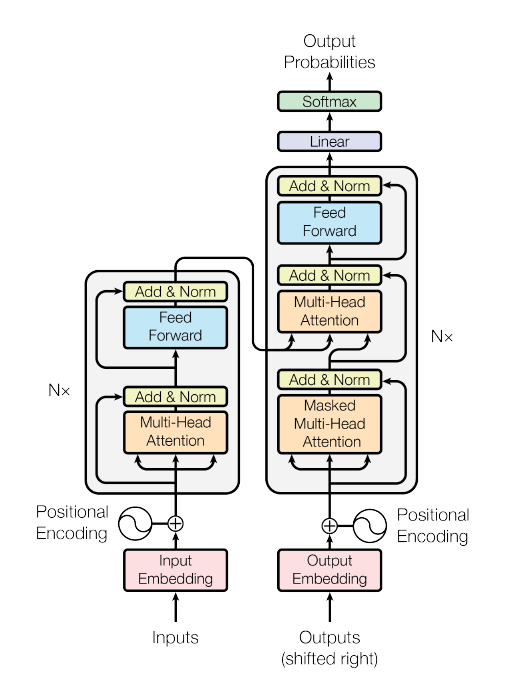
\includegraphics[width=\textwidth]{images/vanilla-arch.png}
    \caption{}
    \label{fig:vanilla-arch}
\end{subfigure}
\begin{subfigure}[b]{0.4\textwidth}
    \centering
    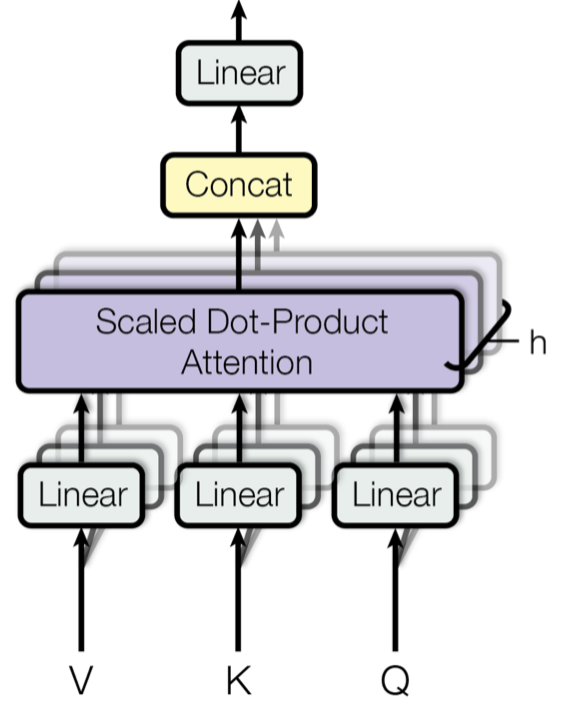
\includegraphics[width=0.9\textwidth]{images/multi-head.png}
    \caption{}
    \label{fig:multi-head}
\end{subfigure}
\caption{Transformers Architecture (a) and Multi-Head Attention (b) \cite{vaswani2023attention}}
\end{figure}

In order to describe the encoder and decoder of the Transformer architecture, we first need to understand the attention mechanisms and position-wise feed-forward layers.

\subsection{Multi-Head Attention}

Attention is the mechanism used by this architecture to capture dependencies between different positions within a sequence by attending to all positions simultaneously. Mathematically, this is represented by the function 
\begin{equation}
    A(Q, K, V) = \softmax\left(\frac{QK^\top}{\sqrt{d_k}}\right) V,
\end{equation}
where $Q \in \mathbb{R}^{m \times d_k}$ is the query matrix, $K \in \mathbb{R}^{n\times d_k}$ is the key matrix, and $V \in \mathbb{R}^{n \times d_k}$ is the value matrix. Conceptually, attention outputs the relevant values given a query to a set of key-value pairs by considering the similarity between the queries and the keys and then obtaining the values corresponding to the most similar keys. The product of $QK^T$ is scaled by $1/\sqrt{d_k}$ due to empirical observations that the unnormalized operation has values in regions of small gradients for the softmax function.

Additionally, to obtain the matrices $Q, K,$ and $V$, generally, an attention mechanism applies a linear map to the inputs $X_Q, X_K,$ and $X_V$, i.e. $Q = X_QW_Q, K=X_KW_K, V=X_VW_V$ for three learnable matrices $W_Q, W_K \in \mathbb{R}^{d \times d_k}, W_V \in \mathbb{R}^{d \times d_v} $. It is the convention to take $d_v = d_k$.


What we just described is called an \textit{Attention Head} and, as the name indicates, the multi-headed attention stacks several attention heads with unique sets of parameters in parallel. The outputs $A_1, \ldots, A_h$ of $h$ heads are then concatenated along the embedding dimension. It is the convention to set $h = d / d_k$ in order to keep the embedding dimension constant throughout the layers for easiness of stacking.

Multi-head attention has three main variants used for the encoder and decoder:
\begin{itemize}
    \item \textbf{Self-Attention:} This is the attention block used for the encoder. It sets $X_Q = X_K = X_V = X$, where $X \in \mathbb{R}^{L \times d}$ is the input of the encoder block.
    \item \textbf{Masked Self-Attention:} This is the first attention block used for the decoder. It also has $X_Q = X_K = X_V = X$ where $X \in \mathbb{R}^{M \times d}$ is the input of the decoder block, but in this variant, the positions are only allowed to attend to earlier positions in the output sequence. This is done by masking future positions to $-\infty$ before the softmax calculation.
    \item \textbf{Encoder-Decoder Attention:} This is the second attention block used for the decoder. It takes as input $X_Q$ the output of the masked self-attention (after residual connection and normalization as discussed later) and $X_K = X_V = Z$, the output of the encoder stack. This is meant to add the context of the input sequence to the decoder.
\end{itemize}


\subsection{Position-Wise Feed-Forward Network}

Attached to the output of the attention mechanisms, the Transformer architecture also includes a fully connected feed-forward network applied to each position of the input sequence separately but with the same weights. It consists of two linear layers connected by a ReLU activation. The inner-dimension is denoted by $d_{ff}$ and is generally taken as $d_{ff} = 4d$. It can still be represented by tensordot operations as:
$$
FFN(X) = ReLU(XW_1 + b_1)W_2 + b_2.
$$ 

Notice that while the attention mechanisms described above capture dependencies between positions, this block embeds positions independently.

\vspace{2em}

Now that we have introduced the two main components, we can describe the full architecture. As represented in figure \ref{fig:vanilla-arch}, both the encoder and decoder are composed of $N$ layers of identical blocks stacked. They have \textit{Add \& Norm} sub-blocks, which represent a residual connector with the input of the preceding block, followed by layer normalization \cite{ba2016layer}. After each multi-head attention of the position-wise feed-forward layer, an Add \& Norm layer is attached.
\begin{itemize}
    \item \textbf{Encoder Block:} Consists of a multi-head self-attention mechanism and a position-wise feed-forward layer.
    \item \textbf{Decoder Block:} Consists of a multi-head masked self-attention mechanism, a multi-head encoder-decoder attention mechanism as described above, and a position-wise feed-forward layer.
\end{itemize}

Although it remains to describe a few components, the key components that will be further explored during this report are highlighted until now: Attention, Encoders, and Decoders.

As for the remaining components, we first have the tokenization. It consists of the process of turning input text into raw atomic data. These raw data
correspond to the basic elements from which the model estimates meaningful interactions.
This is done by assigning an identifier to a word, a character within words or segment
of words (subwords). Starting from a large corpus of text, the tokenizer extracts the
subwords, or tokens, to use for id assignation. As a result, it retrieves a map that relates
tokens with ids. Afterwards, this map is used to tokenize sentences that serve as inputs
to the model.

Once all data is tokenized, we have embeddings for inputs and outputs (inputs for decoder) that transform the tokens to vectors of dimension $d$ with linear transformations. This embedding is added to a positional encoding to inject information about position of tokens. These are then ready to be fed to the model.

Finally, to obtain a probability distribution for the predicted next token of the sequence, the output of the last decoder layer is passed through a linear layer with softmax activation.

\subsection{Model Adaptation}

Generally, the usage of the Transformers architecture we just described can be divided into three different categories:
\begin{itemize}
    \item \textbf{Encoder-Decoder:} The full Transformer architecture. This is typically used for seq-to-seq tasks such as machine translation. 
    \item \textbf{Encoder-only:} Only the encoder part of the Transformer architecture is used, and the encoder output is generally used to embed the input sequence. This is generally used for classification tasks. Notably, the BERT \cite{devlin2019bert} family of models is an example of this.
    \item \textbf{Decoder-only:} Only an adapted decoder is used, with the removal of the Encoder-Decoder attention mechanism. This is commonly used for generative tasks. Notably, the GPT \cite{brown2020language} family of models used a decoder-only architecture.
\end{itemize}

Beyond architectural changes, a great variety of Transformer-based models introduce diverse modifications to the model pipeline. Remarkably, since the Transformer is a flexible architecture and makes few implicit prior assumptions on the input data distribution, it is generally hard to train a model on small-scale data. This issue has been widely tackled by self-supervised pre-training on large datasets \cite{devlin2019bert}\cite{brown2020language}, which allows large networks to be trained without the need to acquire expensive manually labeled data, e.g. in the case of NLP tasks. 

Two classes of pre-training tasks that have been successfully used are \textit{Fill the Blanks} and \textit{Contrastive Learning}. For the former, the task is to predict a hidden or masked part of the input sequence or reverse a permutation applied to the input, which aims to teach the model bidirectional context leveraging. The latter consists of presenting the model with three inputs, two of which are "compatible" and one other that is not; the task is then for the model to detect which two of the three are compatible. This is generally implemented by applying a transformation to the data that is desirable for the model to be invariant. An example of it is \textit{Next Sentence Prediction} which is used for BERT, which helps capture sequence-to-sequence relationships. 

In the era of Large Language Models (LLMs), pre-trained models became the standard. A single general-purpose pre-trained model on large-scale data can be leveraged by fine-tuning the model for a wide-variety of downstream tasks, which has been powering many of the industry applications of NLP.

\subsection{Computational Costs}
Now, let us analyze the computational costs of transformers. We will restrict the study to a single encoder block, for the sake of simplicity, however it easily extends to the decoder block and a stack of blocks of either. Let us use the same notation as before, with an input sequence of length $L$, embedded space of dimension $d$, $h$ attention heads, embedding space for the keys $d_k$ ($d_k h = d$), and let $M$ be the length of the output embedding. The layer normalization and residual connection have linear complexity for each head, thus both memory and computational complexity is $O(h d_k L + Ld) = O(Ld)$.

\begin{table}[ht!]
\centering
\begin{tabular}{l c c} 
 \hline
    Module & Computation & Memory \\ [0.5ex] 
 \hline
 (Masked) Self-Attention & $O(L^2d)$ & $O(Ld + hL^2)$ \\ 
 
 Encoder-Decoder Attention & $O(LMd)$ & $O(Md + hLM)$ \\
 
 FFN & $O(Ld^2)$ & $O(Ld)$ \\

 \hline
\end{tabular}
\caption{Complexity of Attentions and Position-Wise Feed-Forward}
\label{table:1}
\end{table}

Moreover, both the self-attention and position-wise feed-forward have complexities dominated by matrix multiplications. For the former, the multiplication of $\softmax(QK^\top / \sqrt{d_k})$ of shape $L \times L$  with $V$ of shape $L \times d_k$ takes $O(L^2d_k)$ operations and $O(Ld_k)$ to store the result, while computing $QK^\top$ also takes $O(L^2d_k)$ operations and requires $L^2$ of memory to store the result. Repeating this over the $h$ heads gives the complexities as described in table \ref{table:1}. Note that this simply extends to masked self-attention as the operations are essentially the same, and similarly to encoder-decoder attention.

For the position-wise feed-forward layers, assuming the convention that $d_{ff} = 4d$, the tensor-dot described before only requires $O(Ldd_{ff}) = O(Ld^2)$ operations, with $O(Ld)$ memory is sufficient to store the partial results.



\vspace{0.5em}

Now that we analyzed the costs of a single pass through a transformer layer, let us recall that during \textit{inference} we generate one token at a time. This adds a degree to the final computational order of magnitude resulting in $O(LM^2d + M^3d)$ complexity as the decoder has two types of attention. This issue can however be mitigated through clever re-utilization of computations of the previous steps, as formulated in   appendix \ref{sec:appendix}.

\vspace{0.5em}

It is important to remark that this represents the total number of computations per layer, however, these can be efficiently parallelized due to basically no sequential dependency of computations within each module. This is in stark contrast with recurrent networks, which can be argued to have better total complexity but have a higher number of sequential operations.

Moreover, although Transformers improve training speed drastically through improved parallelism, the Self-Attention module has an alarming quadratic complexity in relation to the length of the sequence in both computation and memory. 
This is prohibitive for handling large corpus of text such as codebases, articles, or books, and generally limits the scalability of the architecture. 
Although the overall architecture also has a quadratic number of computations with relation to the embedding dimension $d$, this is a constant set as a hyperparameter, while the input sequence length can be variable and for modern applications it usually holds that $L_{max} \gg d$. With this in mind, a wide variety of novel approaches have been proposed in recent years for efficient architectural modifications. Notably, we will explore two techniques for such: Linear Transformers and Quantization.

\section{Linear Transformers}
\subsection{Theoretical Description}
We follow the theoretical derivations of \cite{katharopoulos2020transformers}. Let $x \in \mathbb{R}^{N \times F}$ be our input (sequence length $N$ and $F$ features). A transformer layer is a function $T \colon \mathbb{R}^{N \times F} \to \mathbb{R}^{N \times F}$ such that 
\begin{gather*}
     Q = xW_Q, K = xW_K, V = xW_V \\
    A(x) = softmax(QK^\top / \sqrt{D}) V \\
    T(x) = f(A(x) + x)
\end{gather*}
for $f$ a feature-independent FFN and projection matrices $W_Q, W_K \in \mathbb{R}^{F \times D}$, $W_V \in\mathbb{R}^{F \times M}$.

If we analyze the complexity of such transformer layer, we notice that the only computation with $O(N^2)$ complexity w.r.t $N$ is the attention layer $A(x)$ with computational complexity $O(N^2(M + D))$ and $O(N^2)$ requirement due to storing $QK^\top$.

To remediate this, a kernalization method is used. Consider a feature map $\phi : \mathbb{R}^D \to \mathbb{R}^C$ (deterministic or not) such that $\exp(\frac{q^\top k}{\sqrt{D}}) \approx \phi(q)^\top \phi(k)$, then we get
\begin{equation}
\label{approx}
    (A(x))_i = \cfrac{\sum_{j=1}^N \exp(Q_i^\top K_j/ \sqrt{D}) V_j}{\sum_{j=1}^N \exp(Q_i^\top K_j / \sqrt{D})} \approx \cfrac{\sum_{j=1}^N \phi(Q_i)^T \phi(K_j) V_j}{\sum_{j=1}^N \phi(Q_i)^\top \phi(K_j)} = \cfrac{\phi(Q_i)^\top \sum_{j=1}^N \phi(K_j)V_j}{\phi(Q_i)^\top \sum_{j=1}^N \phi(K_j)}
\end{equation}
Therefore, $A(x) \approx \phi(Q) (\phi(K)^\top V) / \phi(Q) (\phi(K)^\top 1_N)$ where the division is row-wise and $1_N \in \mathbb{R}^N$ is the vector with all ones. Note that we can compute in $O(NCM)$ operations through the parenthesis indicated precedence. This yields $O(N(C+M))$ memory requirement. 

For the causal masked self-attention variation, we slightly modify \ref{approx} to get
\begin{equation}
    (A(x))_i \approx \cfrac{\phi(Q_i)^\top \sum_{j=1}^i \phi(K_j)V_j}{\phi(Q_i)^\top \sum_{j=1}^i \phi(K_j)} = \cfrac{\phi(Q_i)^\top S_i}{\phi(Q_i)^\top Z_i}
\end{equation}
hence, if we define $S_i := \sum_{j=1}^i \phi(K_j)V_j, Z_i := \sum_{j=1}^i \phi(K_j)$, we can compute $(A(x))_i$ via partial sums in constant operations relative to $N$. Notice that this approach establishes a parallel between linear causal attention and RNNs.

Finally, we can compute the gradients of these approximate linear causal attentions also in linear time and memory with similar partial sums to $S_i, Z_i$. In particular, with the custom gradient computation instead of the auto-grad, we avoid tracking all the $S_i, Z_i$, and instead only using $Q, K, V$. 

The main question that remains is: How to design the feature map to approximate the desired $\sigma$.

\subsection{Paper-specific approaches}

In Transformers are RNNs: Fast Autoregressive Transformers with Linear Attention\cite{katharopoulos2020transformers}, the paper that described the derivations done above, the authors consider a simple feature map $\phi(x) = elu(x) + 1$ due to ease of computation, positiveness, and favorable gradient properties.

\vspace{1em}
 
Random Feature Attention \cite{peng2021random} proposes a randomized feature function 
$$
\phi(x) = \sqrt{1/L} \Bigl[ \sin(w_1 \cdot x), \ldots, \sin(w_L \cdot x), \cos(w_1 \cdot x), \ldots \cos(w_L \cdot x) \Bigr]^\top
$$
for $D$-dimensional random vectors $w_i \sim \mathcal{N}(0, \lambda^2 I_L) $. The motivation comes from $\mathbb{E}[\phi(x)^T \phi(y)] = \exp(- \| x - y \|^2 / 2\lambda^2)$ so if we normalize the queries and keys to unit vectors, we get $\exp(q^\top k /\lambda^2) \propto \phi(q)^\top \phi(k) $ (in expectation).

Moreover, it also introduces a gating mechanism inspired by RNN's to the causal attention scenario with the goal of learning with recency bias.

\vspace{1em}

Rethinking Attention with Performers \cite{choromanski2022rethinking}, on the other hand, proposes another two random feature functions $$\phi_1(x) = \exp(-\|x\|^2/2)(\exp(w_1 \cdot x) + \ldots \exp(w_m \cdot x))$$  $$\phi_2(x) = \frac{1}{\sqrt{2}}\exp(-\|x\|^2/2)(\sum_{i=1}^m \exp(w_i \cdot x) + \exp(-w_i \cdot x))$$ with $w_i$ being sampled either from $\mathcal{N}(0, I_D)$ or to a uniform distribution over the sphere of radius $\sqrt{D}$ in $\mathbb{R}^D$. Additionally, the authors propose to entangle the random samples $(w_i)_1^m$ to be orthogonal for variance reduction. Finally, substituting $\exp$ by $ReLU$ in the equations above also yields good results empirically.

These methods are all proved to approximate the softmax attention mechanism and in comparison with the feature function suggested by \cite{peng2021random}, these provide more desirable numerical properties due to positivity everywhere, which results in more stable and strong performance in selected benchmarks.

\vspace{1em}

Linear Transformers are Secretly Fast Weight Programmers \cite{schlag2021linear} proposes a deterministic feature function to address the variance introduced by the random sampling of the models cited before. It then introduces $\phi$ defined by concatenating \begin{equation}\label{FWP}\phi_{i, v}(k) = ReLU([k, -k]^\top)_i ReLU([k, -k]^\top)_{i + v}\end{equation} for $i \in [1, 2D]$, $v \in [1, \nu]$ (indices taken modulo $2D$).

Moreover, it also introduces a modified update rule for the causal attention partial sums as done on \ref{approx}, a "memory gating mechanism", that empirically shows improvements not only for the author's choice of kernel, but also for RFA\cite{peng2021random} and Performers\cite{choromanski2022rethinking}.

\vspace{1em}
EcoFormer: Energy-Saving Attention with Linear Complexity \cite{liu2023ecoformer} introduces yet another approach to the kernalization by using a learnable binary hash function $\phi(x) \in \{-1, 1\}^b$. With the $b$-bit binary representation, the expensive floating point multiplications and accumulations can be expressed as fast bit-wise operations. This hash function is obtained via self-supervised learning to preserve the relationship information between queries and keys.

\section{RWKV: Reinventing RNNs for the Transformer Era \cite{Peng2023}}

The authors of RWKV have an alternative formulation for linear attention transformers, although it is also motivated by RNNs.

Inspired by \cite{Zhai2021}, the authors opt for an alternative formulation of attention as
$$
    \text{Attn}^+ (W, K, V)_t = \frac{\sum_{i=1}^t \exp(w_{t, i} + k_i) \odot v_i}{\sum_{i=1}^t \exp(w_{t, i} + k_i)}
$$
with $w_{t, i} = -(t - i - 1)w$ for $i \leq t - 1$ and $w_{t, t} = u$, where $w$ represents a positional weight decay ($w \in \mathbb{R}_{\geq 0}^d$) and $u$ is a separate vector that attends exclusively to the current token. Heuristically, by replacing $Q$ by $W$, we establish a linear measure "similarity".

From that, the authors define two sub-blocks of the RWVK block:
\begin{itemize}
    \item \textbf{Time Mix Block:} This block is analogous to the attention block of vanilla Transformers. It can be expressed by 
    \begin{align*}
        r_t &= W_r \cdot (\mu_r \odot x_t + (1 - \mu_r) \odot x_{t-1}), \\ 
        k_t &= W_k \cdot (\mu_k \odot x_t + (1 - \mu_k) \odot x_{t-1}), \\ 
        v_t &= W_v \cdot (\mu_v \odot x_t + (1 - \mu_v) \odot x_{t-1}), \\ 
        o_t &= W_i \cdot (\sigma(r_t) \odot \text{Attn}^+ (W, K, V)_t),
    \end{align*}
    where $x_t$ is the input after a layer normalization of the block, and $x_{t-1}$ is the respective input of the previous layer.
    Notice that in these equations are roughly equivalent to an LSTM with an attention mechanism added.
    \item \textbf{Channel Mixing Block:} This block is analogous to the FFN block of vanilla Transformers. It can be expressed by:
    \begin{align*}
        r'_t &= W_{r'} \cdot (\mu_{r'} \odot y_t + (1 - \mu_{r'}) \odot y_{t-1}), \\ 
        k'_t &= W_{k'} \cdot (\mu_{k'} \odot y_t + (1 - \mu_{k'}) \odot y_{t-1}), \\ 
        o'_t &= \sigma(r'_t) \odot (W'_v \cdot \max(k'_t, 0)^2).
    \end{align*}
\end{itemize}

These two mechanisms combined allow for
\begin{itemize}
    \item Transformers-like parallelizable training.
    \item RNN-like inference, due to the recursive structure to compute state $t$ based on state $t-1$ without redundant computations.
    \item Linear computational and memory complexity of  $O(NF^2), O(NF)$, respectively. (where input $x \in \mathbb{R}^{N \times F})$.
\end{itemize}

Although this approach needs more testing, on the experiments included by the authors the results are much more promising than all methods included above. In fact, it beats vanilla transformers in most of them.

Notice that it still has some of the problems of other linear transformers, most importantly the information bottleneck due to linearity.


\newpage
\bibliographystyle{plain}
\bibliography{main}

\newpage
\appendix
\section{Appendix}
\label{sec:appendix}

\end{document}
